\documentclass[conference]{IEEEtran}
\usepackage[utf8]{inputenc}
\usepackage{graphicx}
\usepackage{amsmath, amssymb}
\usepackage{subfig}
\usepackage{hyperref}
\usepackage{cite}
\usepackage{xcolor}
\usepackage{listings}
\usepackage{enumitem}
\usepackage{float}
\usepackage{tikz}
\usepackage{booktabs}



% dash-style bullets for itemize
\renewcommand{\labelitemi}{--}
\renewcommand{\labelitemii}{--}
\renewcommand{\labelitemiii}{--}
\renewcommand{\labelitemiv}{--}

% simple code styles (optional)
\definecolor{codegreen}{rgb}{0,0.6,0}
\definecolor{codegray}{rgb}{0.5,0.5,0.5}
\definecolor{codepurple}{rgb}{0.58,0,0.82}
\definecolor{backcolour}{rgb}{0.95,0.95,0.92}

\lstdefinestyle{mystyle}{
    backgroundcolor=\color{backcolour},
    commentstyle=\color{codegreen},
    keywordstyle=\color{magenta},
    numberstyle=\tiny\color{codegray},
    stringstyle=\color{codepurple},
    basicstyle=\ttfamily\footnotesize,
    breakatwhitespace=false,
    breaklines=true,
    captionpos=b,
    keepspaces=true,
    numbers=left,
    numbersep=5pt,
    showlines=false,
    showspaces=false,
    showstringspaces=false,
    showtabs=false,
    tabsize=2
}
\lstset{style=mystyle, showlines=false}
\setlist{leftmargin=*}

\title{Lung cancer segmentation by using Deep Learning}

\author{
Doan Duy Thanh, Le Viet Hoang Lam, Chau Tuan Minh,\\
Hoang Nguyen Tuan Nghia, Nguyen Minh Dat, Duong Tuan Kiet\\
\textit{University of Science and Technology of Hanoi (USTH)}\\
Lecturer: Tran Giang Son
}

\date{Hanoi, March 2026}

\begin{document}
\pagestyle{plain}

\maketitle
\begin{abstract}
Lung cancer remains a leading cause of death worldwide, necessitating early and accurate detection of lung nodules. Computed tomography (CT) is the primary diagnostic tool; however, manual assessment by radiologists is time-consuming and prone to bias between observers. This final report presents an automated framework for detecting and segmenting lung nodules, specifically designed to support Lung-RADS assessment. We propose two modern deep learning architectures: Mask Region Convolutional Neural Networks (Mask R-CNN) and You Only Look Once (YOLO) for rapid identification of nodules within a mass. We have learned how to utilize the method to process and understand the nature of the disease to aid in more accurate nodule identification.
\end{abstract}

\section{Introduction}
Lung cancer is one of the most serious and common types of
cancer worldwide, both in number of new patients
and in number of fatalities. There were an estimated
1.8 million new cases of lung cancer worldwide in 2015~\cite{Siegel2017}.
In the United States in 2020, a total of 228{,}820 new cases of lung cancer
and 140{,}730 deaths were reported, accounting for 36\% of all cancer-related deaths~\cite{Siegel2020}. According to Torre~\cite{Torre2016}, early-stage detection, particularly when the tumor is localized, dramatically increases the patient's survival rate.


Computer-aided diagnosis (CAD) systems are developed to support physicians and radiologists in detecting and diagnosing lung nodules. Typically, CAD for lung cancer includes two main components: a detection module (CADe) and a diagnostic module (CADx)~\cite{LungRADS}. The CADe system focuses on distinguishing pulmonary nodule candidates from non-nodules (such as normal anatomical structures), while CADx evaluates the identified nodules to determine whether they are benign or malignant~\cite{Doi2007}. Because of this design, achieving high accuracy in lung nodule classification is essential to the effectiveness of a CADe system.

Nowadays, deep learning has emerged as the state-of-the-art solution for numerous computer vision tasks, particularly in medical image analysis. Convolutional Neural Networks (CNNs) have proven highly effective in extracting complex spatial features from medical scans. Specifically, in the realm of object detection, architectures such as You Only Look Once (YOLO) and Mask Region Convolutional Neural Networks (Mask R-CNN) have demonstrated exceptional performance. While Mask R-CNN excels in providing precise localization and segmentation of small, subtle objects through its region proposal mechanisms and mask prediction branch, YOLO offers a highly efficient, single-stage detection framework. These advances in deep learning make it highly promising for lung nodule detection and classification systems. 

In the final report, we study the problem of segmenting the nodules of lung cancer. Our objective was to detect lung tumors using the given data. Superior to traditional CNNs, region-based architectures such as Mask R-CNN have set a standard for accuracy in medical imaging. Mask R-CNN utilizes Region Proposal Networks (RPNs) to identify potential lung nodule candidates with high sensitivity, which is crucial for clinical diagnostic workflows.



\section{Related Works}
Object Detection and Segmentation has been significantly propelled by the advancement of Deep Learning. Beyond traditional CNNs, region-based architectures such as Faster R-CNN have established a benchmark for precision in medical imaging. Mask R-CNN utilizes a Region Proposal Network (RPN) to identify potential lung nodule candidates with high sensitivity, which is vital for clinical diagnostic workflows~\cite{He2017}. Conversely, the You Only Look Once (YOLO) framework revolutionized the field by framing detection as a single regression problem, offering remarkable inference speed while maintaining competitive accuracy~\cite{Ultralytics2025}.


In the field of lung cancer research, several groundbreaking studies, such as the research by Associate Professor Tran Giang Son~\cite{Tran2019}, have explored the optimization of deep architectures for the classification and detection of lung nodules. Their work often emphasizes the importance of custom-built models to handle the high variability of nodule morphology in CT images.

Expanding on these existing methodologies, we implement a dedicated 2D detection and segmentation framework designed for Lung-RADS assessment. We leverage custom-built YOLO and Mask R-CNN architectures, trained on the Kaggle lung cancer dataset~\cite{Armato2015}, to achieve high-precision localization of pulmonary nodules.

\section{Materials and Methods}
\subsection{Dataset}
The dataset used is the LIDC-IDRI dataset, which is publicly available on Kaggle~\cite{Armato2015}. This dataset is a specialized lung cancer segmentation collection, meticulously labeled according to the Lung-RADS. This dataset represents a fusion of two primary sources: original local clinical data from the Kazakh Research Institute of Oncology and Radiology and the internationally recognized Lung Image Database Consortium and Image Database Resource Initiative (LIDC-IDRI) dataset. To ensure its utility for standardized clinical reporting, the entire collection has been labeled by expert radiologists to align with Lung-RADS.
The complete dataset utilized in this research comprises 972 CT images, which have been partitioned into a training set of 708 images and a testing set of 264 images. This dataset integrates clinical data from local sources and the LIDC-IDRI database, all re-labeled according to the Lung-RADS system to ensure clinical relevance. Each clinical case is provided with a standardized labeling format consisting of the following components:

\begin{itemize}
    \item \textbf{Lung-RADS Class:} Categorical labels representing the clinical assessment and malignancy risk levels.
    \item \textbf{Binary Mask:} Detailed ground-truth segmentations of the lung cancer area for voxel-level analysis.
    \item \textbf{hu Arrays:} Standardized CT images converted to Hounsfield Units (HU) to represent tissue density accurately.
\end{itemize}

To facilitate efficient model training and reduce computational noise, the dataset includes processed images (\texttt{hu\_array}). In these images, non-lung anatomical structures have been removed via a thresholding-based algorithm, allowing the custom-built models to focus exclusively on the pulmonary regions. This preprocessing step is vital for improving the convergence rate and detection precision of our deep learning architectures.
All input CT images are resized to a resolution of $512 \times 512$ pixels to ensure consistency across the dataset. Prior to being fed into the deep learning models, the CT image intensity is normalized using a Hounsfield Unit (HU) windowing technique specifically designed to highlight anatomical structures within the lung parenchyma. This normalization is implemented via the \texttt{window\_hu()} function using a window center ($C$) of $-600$ and a window width ($W$) of $1500$. 
\begin{figure}[ht] 
    \centering
    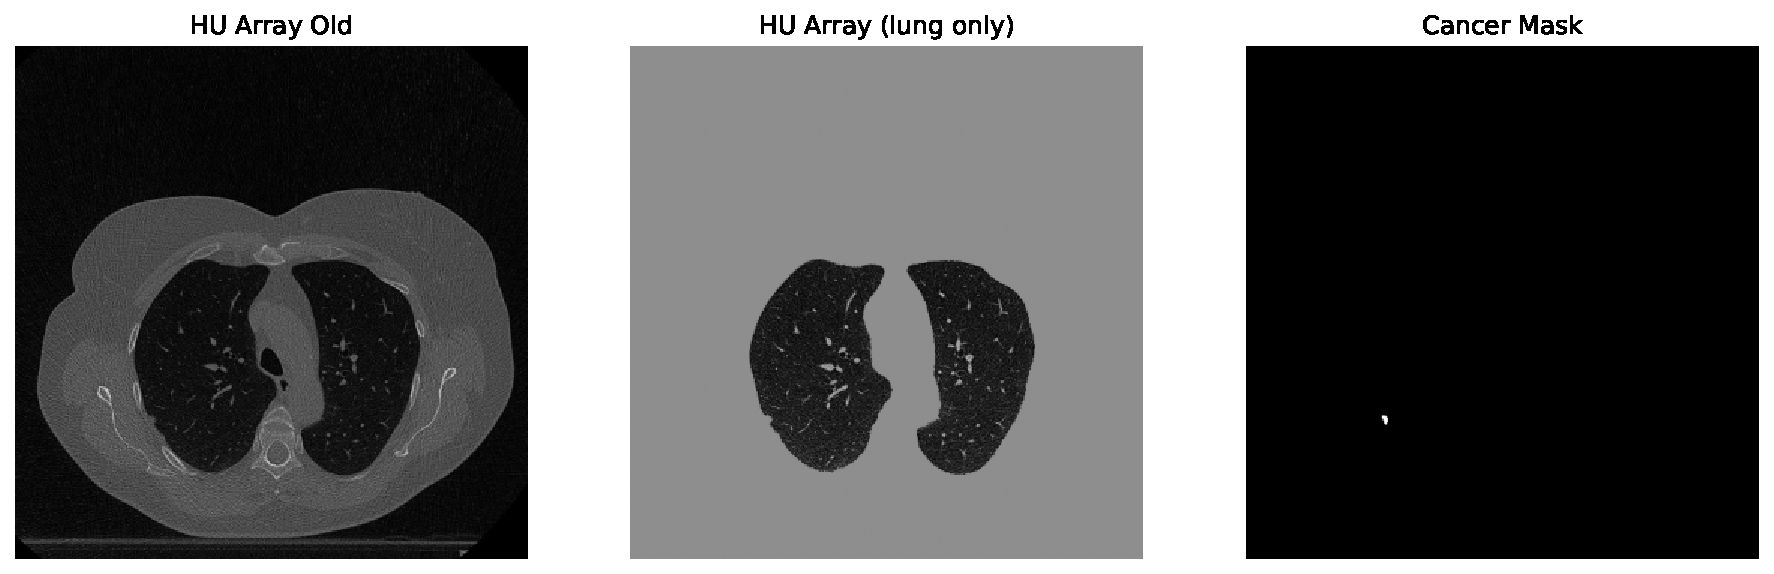
\includegraphics[width=0.48\textwidth]{images/lung_sample_visualization.pdf}
    \caption{Sample visualization of the LIDC-IDRI dataset}\label{fig:sample}
\end{figure}
\subsection{Proposed Model Architectures}
Nowadays, deep learning technique is very strong and has been widely used in many fields. In this final report, we evaluate two distinct deep learning architectures for lung segmentation: a two-stage Mask R-CNN and a single-stage YOLOv8/26. Both models are trained on the same dataset to ensure a fair comparison of their performance in lung nodule detection and segmentation.
\subsection{Mask R-CNN Architecture}
Mask R-CNN, as proposed by Kaiming He~\cite{He2017}, extends Faster R-CNN by adding a branch for predicting an object mask in parallel with the existing branch for bounding box recognition. Mask R-CNN is simple to train and adds only a small overhead to Faster R-CNN, running at 5 fps, good for segmentation tasks.

In figure 2, the mask R-CNN architecture consists of a backbone network for feature extraction, followed by a Region Proposal Network (RPN) that generates candidate object proposals. The architecture then includes a RoIAlign layer to precisely extract features for each proposal, which are fed into two parallel branches: one for bounding box regression and classification, and another for pixel-wise mask prediction. 
\begin{figure}[H]
    \centering
    \includegraphics[width=0.48\textwidth]{images/MaskRCNN architectur.pdf}
    \caption{Mask R-CNN architecture}
    \label{fig:mask_rcnn}
\end{figure}

The model is optimized using a multi-task loss function ($L$) that combines objectness, regression, and segmentation losses:

\begin{equation}
L = L_{\text{rpn\_cls}} + L_{\text{rpn\_reg}} + L_{\text{roi\_cls}} + L_{\text{roi\_reg}} + \lambda L_{\text{mask}}
\end{equation}


where $L_{\text{rpn}}$ and $L_{\text{roi}}$ represent the losses for the proposal and detection stages, respectively, while $\lambda L_{\text{mask}}$ accounts for the weighted binary cross-entropy of the segmentation branch.


The training objective combines several losses from different branches:

\begin{itemize}
    \item \textbf{RPN Classification Loss:}
    

\[
    L_{\text{rpn\_cls}} = -\big[y \log(\sigma(z)) + (1-y)\log(1-\sigma(z))\big]
    \]


    where $z$ is the predicted logit and $y \in \{0,1\}$ is the object/background label.

    \item \textbf{ROI Classification Loss:}
    

\[
    L_{\text{roi\_cls}} = -\sum_{c} y_c \log(p_c)
    \]


    with $y_c$ the one-hot ground truth label and $p_c$ the predicted probability.

    \item \textbf{Bounding Box Regression Loss:}  
    Both RPN and detection head use Smooth L1 loss:
    

\[
    \text{SmoothL1}(x) =
    \begin{cases}
    0.5x^2, & |x| < 1 \\
    |x| - 0.5, & |x| \geq 1
    \end{cases}
    \]



    \item \textbf{Mask Loss:}
    

\[
    L_{\text{mask}} = -\big[y \log(\sigma(m)) + (1-y)\log(1-\sigma(m))\big]
    \]


    where $m$ is the predicted mask logit and $y$ is the ground truth mask.
\end{itemize}

The main network uses a \textbf{SimpleBackbone} with 5 convolutional blocks, progressively reducing spatial resolution and increasing feature channels:

\begin{itemize}
    \item \textbf{Block 1:} Conv2d (3$\rightarrow$64), BatchNorm, ReLU — stride 2 $\rightarrow$ 256$\times$256
    \item \textbf{Block 2:} Conv2d (64$\rightarrow$128), BatchNorm, ReLU — stride 2 $\rightarrow$ 128$\times$128
    \item \textbf{Block 3:} Conv2d (128$\rightarrow$256), BatchNorm, ReLU — stride 2 $\rightarrow$ 64$\times$64
    \item \textbf{Block 4:} Conv2d (256$\rightarrow$256), BatchNorm, ReLU — stride 1
    \item \textbf{Block 5:} Conv2d (256$\rightarrow$256), BatchNorm, ReLU — stride 1
\end{itemize}

A redundant bypass connection links Block 3 and Block 5, improving gradient flow and enabling richer feature learning with a total of 8 steps.

For an input of $512 \times 512$, the output feature map size is:



\[
\frac{512}{8} \times \frac{512}{8} = 64 \times 64
\]



This feature map is shared by: Region Proposal Network (RPN), Detection Head Network, and Mask Head Network. Each of these components operates on the same feature map, allowing for efficient multi-task learning without redundant computations. 



\subsection{YOLOv8/26 Instance Segmentation}
The YOLO architecture, as described by Sapkota and Karkee~\cite{Ultralytics2025}, is a single-stage object detection framework that has been adapted for instance segmentation tasks. The architecture consists of a backbone network for feature extraction, followed by a neck that aggregates features at multiple scales. The head of the network is designed to predict bounding boxes, class probabilities, and segmentation masks simultaneously.
\begin{figure}[H]
    \centering
    \includegraphics[width=0.48\textwidth]{images/Detailed-architecture-of-YOLOv8-showcasing-the-backbone-networks-multiple-convolutional_W640.pdf}
    \caption{YOLOv8/v26 architecture for instance segmentation}
    \label{fig:yolo_architecture}
\end{figure}

The main architectural differences between YOLOv8 and YOLO26 lie in the design of their backbone, neck, and detection head.

YOLOv8 uses advanced convolutional blocks, such as C2f modules, in its backbone to extract rich and detailed features from the input image. Subsequently, the features are passed through a feature-fusion network based on FPN and PAN. This structure helps combine features at different scales, allowing the model to detect both small and large objects effectively. YOLOv8 also uses a decoupled detection head, which separates classification and bounding box regression. This separation improves training stability and overall detection performance.

In contrast, YOLO26 focuses more on computational efficiency. Its backbone is simplified to reduce the number of layers and parameters while still keeping important feature extraction ability. The neck uses a lightweight feature fusion mechanism instead of the more complex FPN/PAN structure, which helps reduce computational cost during inference. In addition, YOLO26 uses a direct regression detection head to predict bounding boxes more directly from feature maps. This makes the prediction process simpler and faster.









\section{Experiments and Results}
\subsection{Experimental Setup}
\subsubsection{Data Preprocessing for YOLO models}

To preprocessing  for the YOLOv8/v26 model is designed to transform raw CT data into an optimized image format suitable for deep learning-based segmentation. The dataset consists of lung CT scan slices stored in a serialized \texttt{.pkl} format and loaded as a Pandas DataFrame. Each record includes the original HU array, a lung-segmented array, and a binary cancer mask.
\begin{enumerate}
    \item \textbf{Intensity Windowing and Normalization:} 
    Since CT images represent pixel intensities in Hounsfield Units (HU) with a wide dynamic range, an intensity windowing technique is applied to highlight specific tissues. The window bounds are calculated as follows:
    
    \begin{equation}
    low = C - \frac{W}{2}, \quad high = C + \frac{W}{2} 
    \end{equation}
    
    where $C$ represents the window center, $W$ denotes the window width, while $low$ and $high$ are the resulting lower and upper intensity thresholds. HU values outside this range are clipped and normalized to a $[0, 1]$ range.

    \begin{figure}[H]
        \centering
        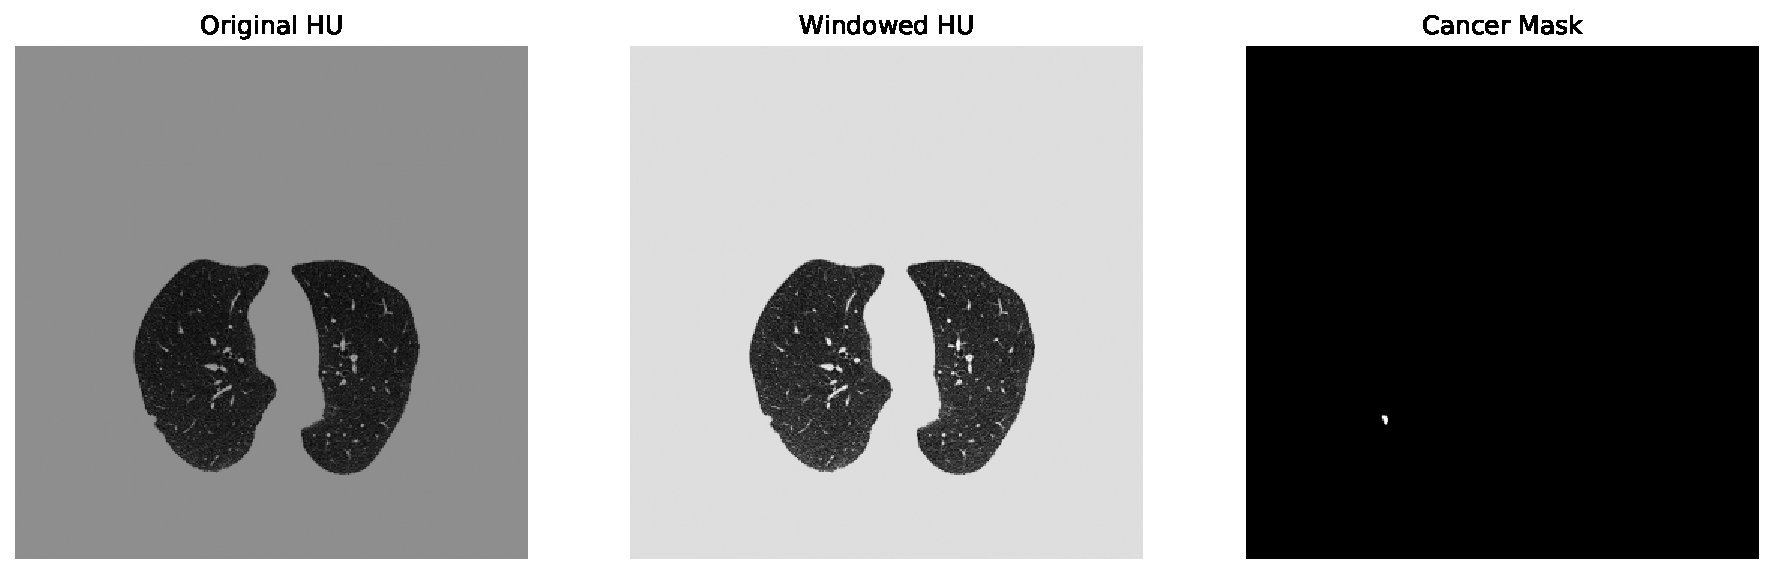
\includegraphics[width=0.48\textwidth]{images/lung_sample_window.pdf}
        \caption{The windowing process: transforming raw CT intensities into a visually interpretable image.}
        \label{fig:windowing_process}
    \end{figure}

    To enhance anatomical representation for YOLOv8/v26, we adopt a multi-window stacking approach. Different window configurations, such as Lung, Soft Tissue, and Bone windows, are stacked to form a three-channel input image.

    \begin{figure}[H]
        \centering
        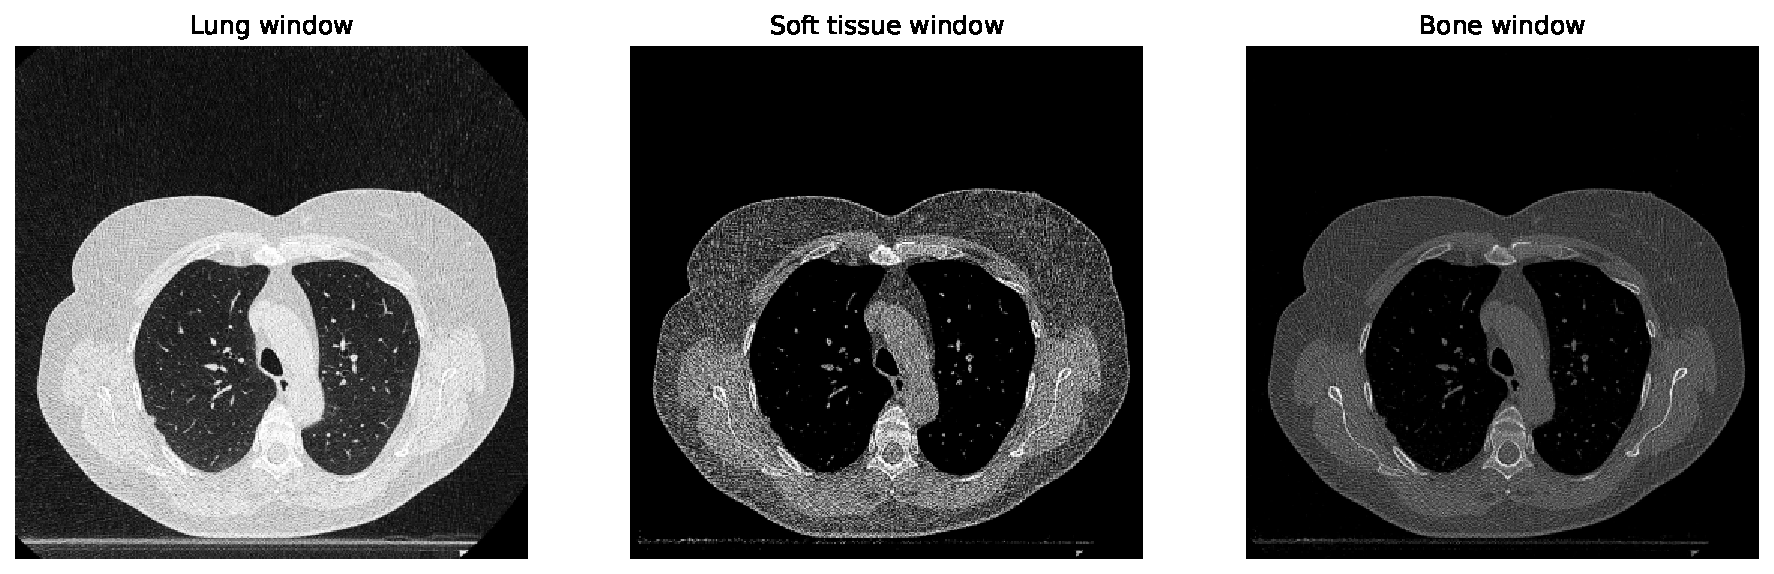
\includegraphics[width=0.48\textwidth]{images/lung_sample_windows.pdf}
        \caption{Multi-window configurations: Lung window, Soft tissue window, and Bone window stacked for multi-channel input.}
        \label{fig:multi_window}
    \end{figure}

    \item \textbf{Polygon Label Conversion:} 
    For YOLOv8/v26 instance segmentation, binary \texttt{mask} attributes must be converted into normalized polygon coordinates. The normalization ensures consistency across different image resolutions:
    
    \begin{equation}
    x_{norm} = \frac{x_{pixel}}{W_{img}}, \quad y_{norm} = \frac{y_{pixel}}{H_{img}} 
    \end{equation}
    
    where $(x_{pixel}, y_{pixel})$ are the original coordinate values from the extracted tumor boundary, while $W_{img}$ and $H_{img}$ denote the width and height of the CT slice, respectively.

    \begin{figure}[H]
        \centering
        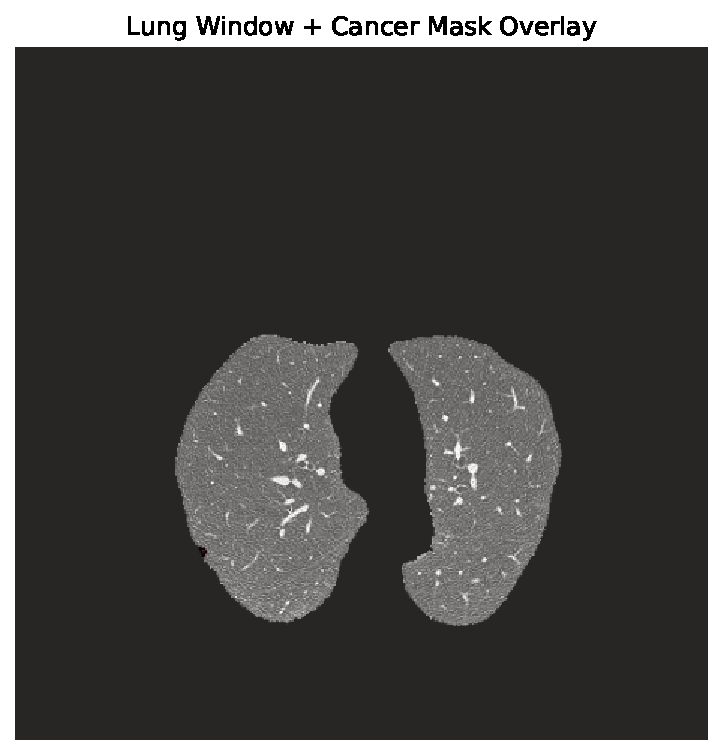
\includegraphics[width=0.28\textwidth]{images/lung_win_mask.pdf}
        \caption{Visualization of polygon label conversion: the cancer segmentation mask overlaid on the lung window.}
        \label{fig:mask_overlay}
    \end{figure}
\end{enumerate}

\subsubsection{Preprocessing for Mask R-CNN model}
To improve the model's learning ability for small lung nodules, the system uses a data enhancement strategy implemented in the Lung Mask RCNN Datasetlayer. Two types of enhancement are applied during training:

Zoom-cropping enhancement. For samples containing lung nodules, the bounding box is extracted from the mask, and then the center of the bounding box is calculated: ($c_x, c_y$):\begin{equation}c_{x}=\frac{x_{1}+x_{2}}{2}, \quad c_{y}=\frac{y_{1}+y_{2}}{2}\end{equation}

where $(x_1, y_1)$ and $(x_2, y_2)$ represent the top-left and bottom-right coordinates of the bounding box, respectively. From this center, a square window is cropped out with a random border. The border is selected from the set: {80, 96, 112, 128, 160}. The cropped image and mask are then resized back to 512×512 using nearest-neighbor interpolation. After resizing, the bounding box is recalculated from the new mask. This strategy allows the model to observe the same lung nodule at different scales, thereby improving learning ability on smaller lesions.

Random flipping. In addition to cropping the image when zoomed in, two geometric improvements are applied:
Random horizontal flipping with a probability of 0.5 and random vertical flipping with a probability of 0.5

When applying the flipping operation, both the image and the mask are flipped accordingly, and the bounding box is recalculated from the flipped mask to ensure spatial consistency.
\begin{figure} [h]
    \centering
    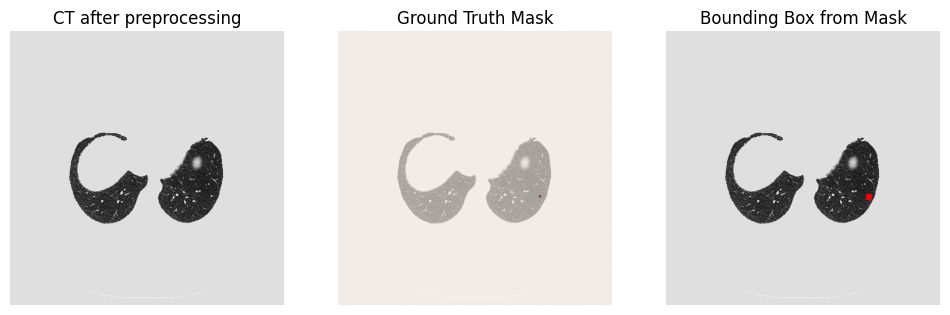
\includegraphics[width=0.48\textwidth]{images/5.png}
    \caption{Data augmentation strategies for Mask R-CNN training.}
    \label{fig:data_augmentation}
\end{figure}


\subsubsection{Performance Metrics}    


Dice Score (the ability to measure the spatial similarity between the predicted and ground truth masks), Intersection over Union or IoU (the ability to quantify the overlap area between masks), mean Average Precision at 0.50 or mAP@0.50 (the ability to determine the detection accuracy at a 0.50 IoU threshold), Recall (the ability to determine the proportion of actual nodules correctly identified), and Precision (the ability to determine the proportion of positive identifications that were actually correct) are used to measure the correctness of the segmentation and detection tasks. These metrics are widely used in medical imaging and are defined as follows:

\begin{equation}
Dice = \frac{2 \times |B_{pred} \cap B_{gt}|}{|B_{pred}| + |B_{gt}|}
\end{equation}

\begin{equation}
IoU = \frac{|B_{pred} \cap B_{gt}|}{|B_{pred} \cup B_{gt}|}
\end{equation}

\begin{equation}
mAP@0.50 : IoU \geq 0.50
\end{equation}

\begin{equation}
Recall = \frac{TP}{TP + FN}
\end{equation}

\begin{equation}
Precision = \frac{TP}{TP + FP}
\end{equation}

where $B_{pred}$ represents the predicted mask generated by the model and $B_{gt}$ is the ground truth mask. For image slices containing multiple nodules, all individual ground truth masks are merged into a single binary mask before comparison to ensure evaluation consistency. Regarding the detection components, TP (true positive) represents the number of lung nodules correctly detected by the model, while FP (false positive) denotes the instances where non-nodule regions are incorrectly identified as nodules. Conversely, FN (false negative) represents the number of actual lung nodules that the model failed to detect during the inference process.



\subsubsection{ Hardware and Software Configuration}
Our experiments are performed on the Google Colab Pro platform to ensure high-performance computing for both training and inference phases. The training tasks, which involve hyperparameter tuning and large-scale image processing, are carried out using NVIDIA A100 Tensor Core GPUs with up to 40 GB of VRAM. This cloud-based environment provides high-memory instances with 51 GB of system RAM and 100 GB of persistent disk storage, allowing for efficient management of the serialized \texttt{.pkl} dataset and multi-window image stacking processes.
\subsubsection{Training}

During the training phase of YOLOv8 and YOLO26, the AdamW optimizer is applied with an initial learning rate of 0.0003 and a batch size of 6. The input image resolution is set to 1024 × 1024. Both models are trained for up to 200 epochs, with early stopping (patience = 40) based on the validation loss to prevent overfitting. In practice, the training process stops at epoch 59 for YOLOv8 and epoch 73 for YOLO26, as the validation performance no longer improves beyond these points. The dataset is divided into training and validation sets, and the validation set is used for model selection and performance monitoring.


Mask R CNN was train over 40 epochs with a batch size of 4. In each batch, input images were processed by the backbone to produce feature maps, followed by RPN scoring, bounding-box regression, and proposal generation via Non-Maximum Suppression with ground truth boxes added. RoI features were extracted, then the detection head predicted class logits and bounding-box bias, while the mask head produced segmentation masks for positive RoIs. The total loss was computed, with mask loss weighted   by $\lambda = 2.0$, and parameters updated using backpropagation. Optimization employed AdamW with learning rate $1\times10^{-4}$, weight decay $1\times10^{-4}$, and cosine annealing to gradually reduce the learning rate to $1\times10^{-6}$.  

All parameters of the backbone, RPN, detection head, and mask head were updated simultaneously. The best model checkpoint was selected based on the highest validated Dice score.

\subsection{Results and Discussions}
\subsubsection{Results of YOLOv8/26}
The comparative performance of YOLOv8 and YOLO26 is summarized in Table \ref{tab:yolo_comparison}. The results were obtained from the best-performing epochs during the training phase. 

YOLO26 demonstrates a significantly higher precision of approximately 0.73, indicating a reduction in false positives. Conversely, YOLOv8 achieves a higher recall of 0.62, suggesting a better ability to identify a larger number of nodules within the dataset. The overall detection ability, measured by mAP50, remains consistent across both architectures at approximately 0.61.
\begin{figure}[h]
    \centering
    \includegraphics[width=0.48\textwidth]{images/Blank 2 Grids Collage (2).png} 
    \caption{Comparison of detection results between YOLOv8 and YOLO26.}
    \label{fig:yolo_comparison}
\end{figure}



\begin{table}[htbp]
\centering
\caption{Quantitative performance comparison between YOLOv8 and YOLO26.}
\label{tab:yolo_comparison}
\begin{tabular}{@{}lcc@{}}
\toprule
\textbf{Metric}    & \textbf{YOLOv8} & \textbf{YOLO26} \\ \midrule
Best Epoch         & 13              & 32              \\
Precision          & 0.574           & 0.734           \\
Recall             & 0.623           & 0.549           \\
mAP50              & 0.612           & 0.613           \\ \bottomrule
\end{tabular}
\end{table}





\subsubsection{Results of Mask R-CNN}


\begin{table}[h]
\centering
\begin{tabular}{lc}
\hline
\textbf{Metric} & \textbf{Value} \\ \hline
Dice            & 0.22           \\
IoU             & 0.16           \\
mAP@0.50        & 0.33           \\
Recall          & 0.56           \\ \hline
\end{tabular}
\caption{Quantitative performance of the Mask R-CNN model on the test set.}
\label{tab:maskrcnn_quantitative}
\end{table}

The quantitative performance of the Mask R-CNN model on the test set is summarized in Table \ref{tab:maskrcnn_quantitative}. These results were obtained by loading the best checkpoint, which was selected based on the highest validated Dice score recorded during the training phase. Throughout the training process, various loss components—including RPN objectness, RPN regression, ROI classification, ROI regression, and Mask loss—were monitored. The training curves illustrated a consistent decreasing trend across all functions, indicating that the model successfully learned features for both the proposal generation and the final segmentation stages.

The model achieved a recall score of 0.56, meaning it successfully detected 56\% of lung nodules in the test dataset, while the mAP@0.50 score of 0.33 indicates a reasonable level of detection accuracy. Regarding the segmentation performance, the indices (Dice = 0.22 and IoU = 0.16) show that while the model is capable of locating nodules within the lung parenchyma, the predicted mask shapes still require further refinement to improve boundary precision. 

Qualitative visualizations of these results are presented in Figure \ref{fig:mask_qualitative_results}. For each test sample, the visualization displays the input CT image alongside the ground truth mask (represented in green) and the predicted mask (represented in red). These visual comparisons demonstrate the model's capability to localize and segment nodular regions across various CT slices, providing a clearer understanding of its performance beyond numerical metrics.

\begin{figure}[h]
    \centering
    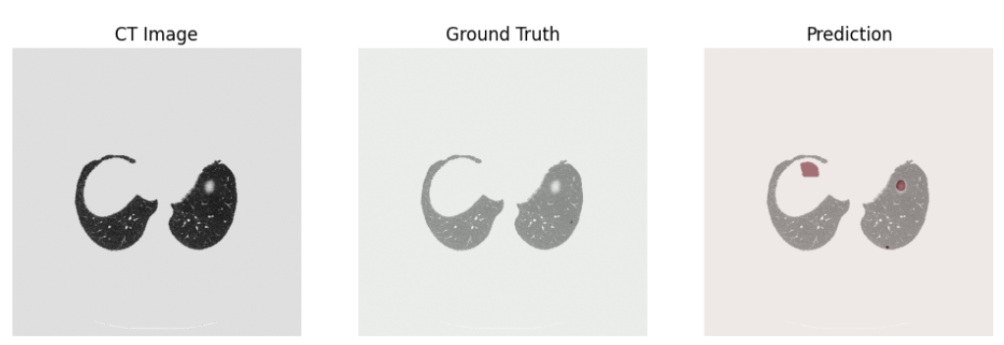
\includegraphics[width=0.48\textwidth]{images/mask_rcnn_qualitative.png}
    \caption{Qualitative segmentation results of Mask R-CNN showing the input CT, ground truth, and predicted masks.}
    \label{fig:mask_qualitative_results}
\end{figure}







\subsubsection{Analysis the training process }
The validation curves show different learning trends for the two models. YOLO26 demonstrates a relatively stable pattern across precision, recall, and mAP throughout the training process, with moderate fluctuations between epochs. In contrast, YOLOv8 exhibits larger variations in these metrics, especially in the recall and mAP curves. Overall, both models show performance improvements during the early training stages, followed by oscillations around a certain range as training progresses.

\begin{figure}[h]
    \centering
    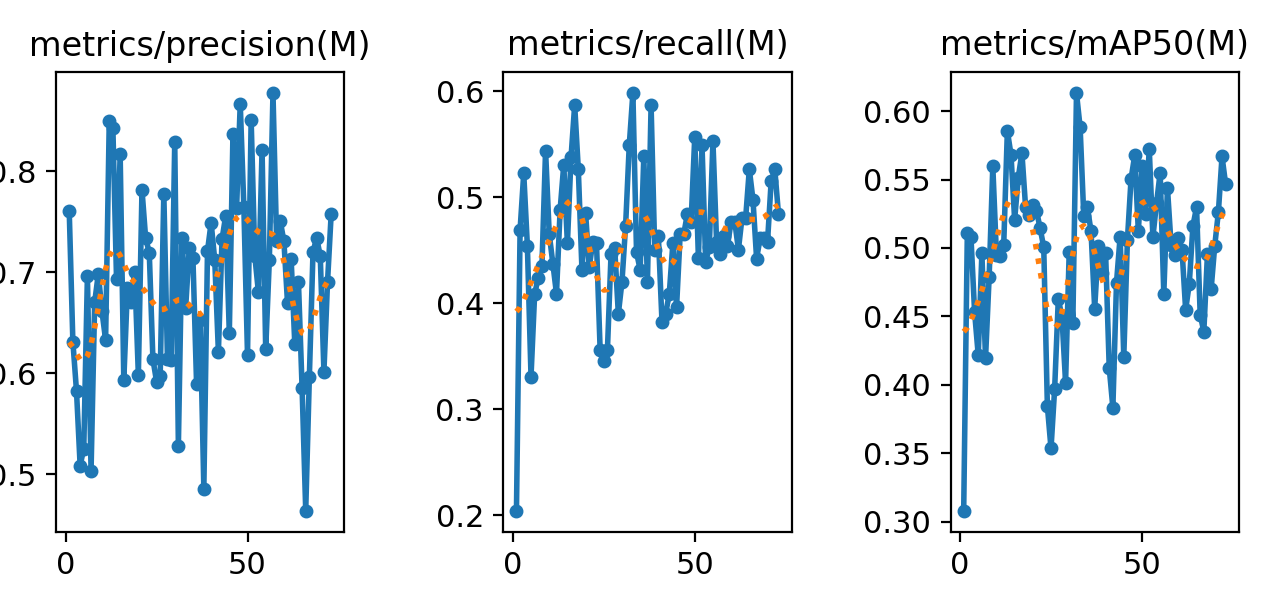
\includegraphics[width=0.48\textwidth]{images/results.png}
    \caption{Evaluate of YOLO26}
    \label{fig:yolo_validation_curve}
\end{figure}

\begin{figure} [h]
    \centering
    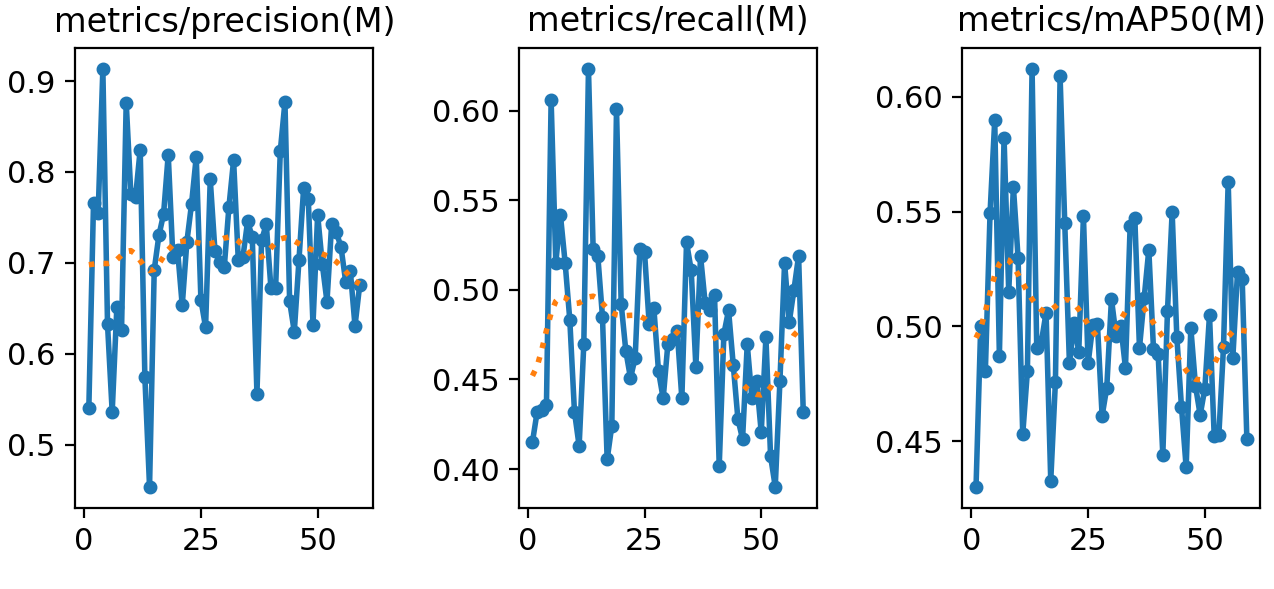
\includegraphics[width=0.38\textwidth]{images/results (1).png}
    \caption{Evaluate of yolov8}
    \label{fig:yolo_validation_curve}
\end{figure}

To assess the modell learning progress, the various components of the multitask loss function comprising RPN objectness, RPN regression, ROI classification, ROI regression, and mask loss were monitored throughout the training process. As illustrated in Figure \ref{fig:training_loss_curve}, the loss values exhibited a gradual decreasing trend as the number of epochs increased, indicating that the model effectively learned useful features from the training data. Notably, the mask loss decreased significantly in the early epochs before stabilizing, which suggests that the segmentation branch of the model successfully began to learn how to predict nodule regions.

\begin{figure}[h]
    \centering
    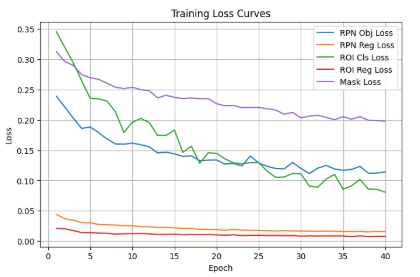
\includegraphics[width=0.38\textwidth]{images/3.png}
    \caption{Training loss curves showing the decreasing trend of multi-task loss components.}
    \label{fig:training_loss_curve}
\end{figure}

 We can see the Dice coefficient and Intersection over Union (IoU) indices on the validation set were tracked to evaluate the quality of the segmentation branch. As shown in Figure \ref{fig:validation_matrix_curve}, although these two indices tended to increase during certain training phases, significant fluctuations occurred between epochs. This phenomenon primarily stems from the inherent characteristics of the lung nodule detection and segmentation task. Specifically, nodules are typically very small relative to the overall CT image, their shapes vary considerably, and the number of positive pixels in the mask is relatively small. Consequently, accurately predicting the nodule boundaries becomes more challenging, leading to the observed instability in Dice and IoU values during training.

\begin{figure}[h]
    \centering
    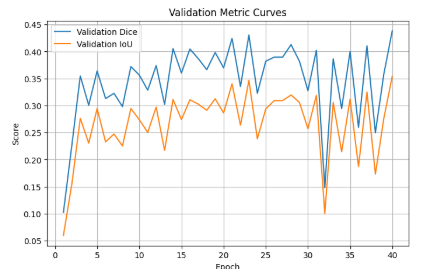
\includegraphics[width=0.38\textwidth]{images/4.png}
    \caption{Validation metrics curves showcasing Dice and IoU fluctuations.}
    \label{fig:validation_matrix_curve}
\end{figure}







\section{Discussion}

The experimental results highlight key differences among YOLOv8, YOLO26, and Mask R-CNN in lung nodule detection and segmentation. YOLO26 achieved higher precision (0.734), showing its simplified design reduces false positives more effectively than YOLOv8 (0.574). In contrast, YOLOv8 reached better recall (0.623), indicating stronger sensitivity to diverse nodule features. Despite these differences, both YOLO-based models maintained similar overall detection capability with mAP@0.50 around 0.61.

Mask R-CNN delivered lower performance, with mAP@0.50 of 0.33 and recall of 0.56. Its training showed unstable Dice (0.22) and IoU (0.16), reflecting the difficulty of segmenting nodules that occupy a very small portion of CT slices and often blend with surrounding lung tissue. The Region Proposal Network struggled to generate consistent candidate regions, which limited the segmentation branch and reduced boundary accuracy.





\section{Conclusion}

We successfully developed and evaluated three deep learning models for automated detection and segmentation of lung nodules on CT images. YOLOv8 and YOLO26 showed better accuracy and efficiency than Mask R-CNN. YOLO26 reduced false positives more effectively, while YOLOv8 achieved higher recall and detected more nodules. Mask R-CNN localized nodules but struggled with mask refinement because nodules are small and vary in shape. The results suggest that one-stage detectors are suitable for fast clinical screening, while segmentation-focused frameworks need further improvement to reach higher boundary precision in medical diagnosis.






\begin{thebibliography}{9}




\bibitem{Siegel2017}
R.~L.~Siegel, K.~D.~Miller, and A.~Jemal,
``Cancer statistics, 2017,''
\textit{CA: A Cancer Journal for Clinicians},
vol.~67, no.~1, pp.~7--30, 2017.

\bibitem{Siegel2020}
R.~L.~Siegel, K.~D.~Miller, and A.~Jemal,
``Cancer statistics, 2020,''
\textit{CA: A Cancer Journal for Clinicians},
vol.~70, no.~1, pp.~7--30, 2020.
\bibitem{Torre2016}
L.~A.~Torre, R.~L.~Siegel, and A.~Jemal,
``Lung cancer statistics,''
in \textit{Lung Cancer and Personalized Medicine},
pp.~1--19, Springer, Berlin, Germany, 2016.
\bibitem{Doi2007}
K.~Doi,
``Computer-aided diagnosis in medical imaging: historical review, current status and future potential,''
\textit{Computerized Medical Imaging and Graphics},
vol.~31, no.~4--5, pp.~198--211, 2007.
\bibitem{LungRADS}
American College of Radiology,
``Lung CT Screening Reporting and Data System (Lung-RADS),''
2014 (updated 2022).
\bibitem{He2017}
K.~He, G.~Gkioxari, P.~Dollar, and R.~Girshick,
``Mask R-CNN,''
\textit{Proceedings of the IEEE International Conference on Computer Vision (ICCV)},
pp.~2961--2969, 2017.


\bibitem{Ultralytics2025}
R.~Sapkota and M.~Karkee,
``Ultralytics YOLO Evolution: An Overview of YOLO26, YOLO11, YOLOv8, and YOLOv5 Object Detectors for Computer Vision and Pattern Recognition,''
Cornell University, Biological \& Environmental Engineering, Ithaca, NY, USA, 2025. [Online]. Available: https://arxiv.org/html/2510.09653v2
\bibitem{Tran2019}
G.~S.~Tran, J.-C.~Burie, T.~P.~Nghiem, V.~T.~Nguyen, and C.~M.~Luong,
``Improving Accuracy of Lung Nodule Classification Using Deep Learning with Focal Loss,''
\textit{Journal of Healthcare Engineering},
vol.~2019, Article ID 5156416, 9 pages, 2019.
\bibitem{Armato2015}
S.~G.~Armato~III, G.~McLennan, L.~Bidaut, M.~F.~McNitt-Gray, C.~R.~Meyer,
``Data From LIDC-IDRI [Data set],''
2015. [Online]. Available: \url{https://www.kaggle.com/datasets/aminasirinechieb/lung-cancer-segmentation-lung-rads}



\end{thebibliography}






\end{document}
